\chapter{The Case\label{case}}

\section{Architecture}
The studied application was build following monolith architecture with three tier pattern containing frontend, backend and database.
The backend was written using node.js version v14.19.1 that uses V8 engine version \textit{8.4.371.23-node.85}.
The backend contains multiple independent components each with its own purpose.
One of the components were refactored out of the monolith application into the independent service.

The independent service contained an application interface to allow communication to the component and the component itself.
The independent service was build using node.js with version v14.18.3 that uses V8 engine version \textit{8.4.371.23-node.85}.
The architecture before and after refactoring can be seen in figures \ref{figure:architecture:monolith} and \ref{figure:architecture:independent_service}.

\begin{figure}
    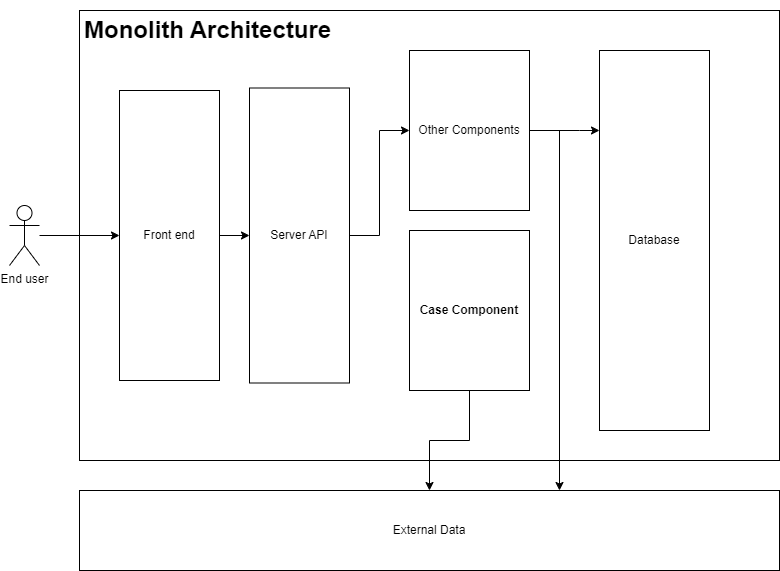
\includegraphics[width=\textwidth]{images/monolith_architecture.png}
    \caption{Architectural overview of the application before refactoring.}
    \label{figure:architecture:monolith}
\end{figure}
\begin{figure}
    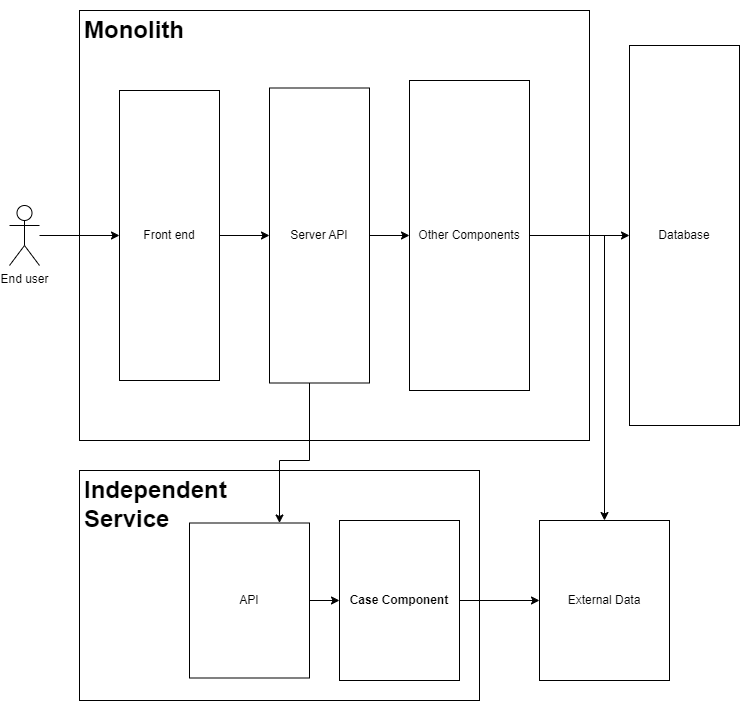
\includegraphics[width=\textwidth]{images/independent_service_arcitecture.png}
    \caption{Architectural overview of the application after refactoring the component into independent service.}
    \label{figure:architecture:independent_service}
\end{figure}

Both environments, the monolith and the independent service, were running in linux server provided by amazon web services.
The hardware specifications were different in both environment.
The monolith environment had 64GB RAM with 8 vCPU of computing power while the independent service had 4GB RAM with 1 vCPU of computing power available.
The use of production environment didn't allow to utilize same resources for both environments.

\begin{table}[h!]
    \begin{tabular}{|c|c|c|c|c|} 
        \hline
        Environment
        & RAM (GB)
        & Core (vCPU)
        & Node.js version
        & V8 version
        \\ 
        \hline\hline
        Monolith
        & 64GB
        & 8
        & v14.19.1
        & 8.4.371.23-node.85
        \\
        Independent service
        & 8GB
        & 1
        & 14.18.3
        & 8.4.371.23-node.85
        \\
        \hline
    \end{tabular}    
    \caption{Hardware specification.}
    \label{represented:harware:specs}
\end{table}

\section{Overview of the Component}
The component was written using javascript with node.js runtime environment.
The component runs in cycles where one cycle contains two to four tasks.
After a cycle is finished the component decides if it start new cycle.
The cycles keeps running until user interrupts the cycles or and error stops the process.

The component is divided into four modules each handling one of the four task.
Each task is represented by its own module and each module is run sequentially one after the other
all of the modules response time is critical to the system.
\begin{itemize}
    \item
    \textbf{Module A} is the first module in the cycle.
    It is always called when the cycles are running.
    
    \item
    \textbf{Module B} is the second module in the cycle.
    It runs after \textbf{module A}.
    
    \item
    \textbf{Module C} is the third module in the cycle.
    It runs after \textbf{module B} only when the response from \textbf{module A} requires it to run.
    Otherwise rest of the modules in the cycle are skipped and the cycle restarts from \textbf{module A}.

    \item
    \textbf{Module D} is the last module in the cycle.
    After it is finished the cycle is restarted from \textbf{module A}.
\end{itemize}

The components is dependent on the input parameters that decides when the component can continue the cycles.
Modules A, C and D are dependent on external data.
Module D is dependent on module C and module C is dependent on module A.
The dependencies of the modules can be seen in figure \ref{figure:module:relation}.
The flowchart of the modules are shown in figure \ref{figure:module:flow}.

\begin{figure}
    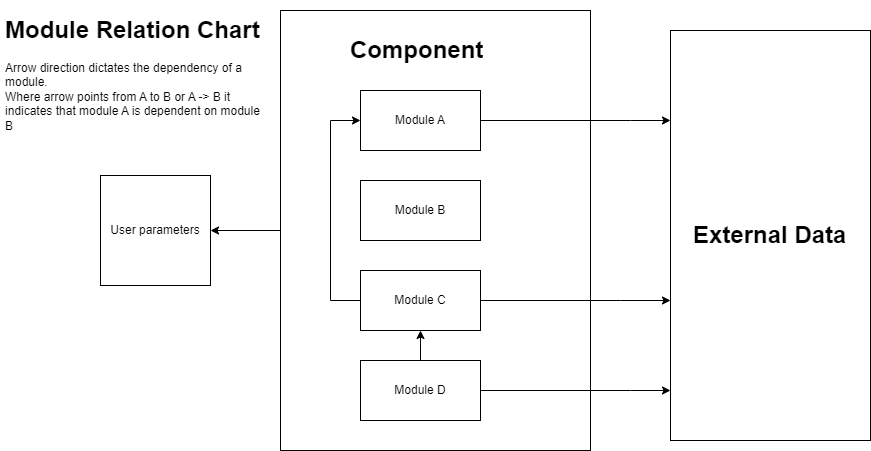
\includegraphics[width=\textwidth]{images/modules_relation_uml.png}
    \caption{Components modules and their dependencies.}
    \label{figure:module:relation}
\end{figure}


\begin{figure}
    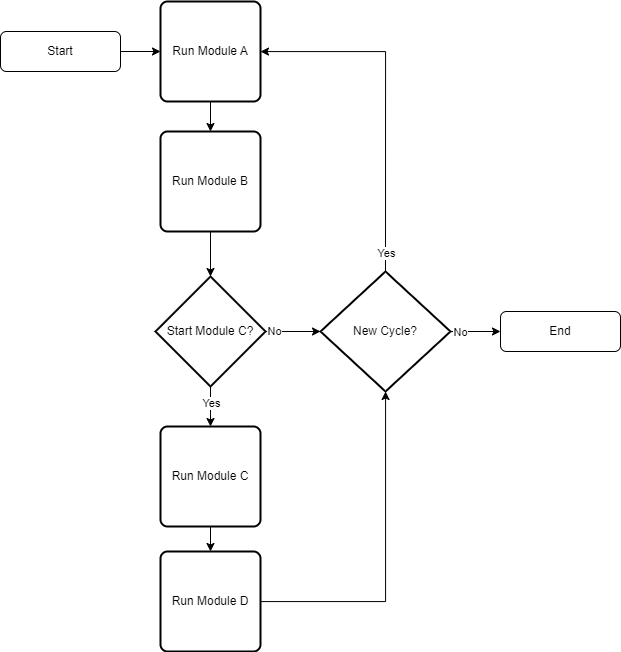
\includegraphics[width=\textwidth]{images/module_flow_chart.png}
    \caption{Modules flowchart. Modules are run inside the studied component.}
    \label{figure:module:flow}
\end{figure}

When any of the modules fails to perform its task an error is raised and the cycle is interrupted.
Error at any point of the cycles requires manual restart from the user.
When modules are running without errors the modules A and B are always performed. 
The modules C and D are run only when the data from module A requires them to run.
Each module waits for the response of external calls before continuing their process.
A full cycle requires successful run from all four modules.
